
\batchmode
\documentclass[10pt]{amsart}
\usepackage{amsmath,amsfonts,amssymb,multicol}
\usepackage{booktabs,tabularx,colortbl,caption,xcolor}
\usepackage{path}
  \discretionaries |~!@$%^&*()_+`-=#{"}[]:;'<>,.?\/abcdefghijklmnopqrstuvwxyzABCDEFGHIJKLMNOPQRSTUVWXYZ0123456789|
\usepackage[pdftex]{graphicx}
\usepackage{epstopdf}  % allows use of eps files with pdftex
\usepackage{epsf}
\usepackage{epsfig}
\usepackage{pslatex}
\usepackage[utf8]{inputenc}
\pagestyle{plain}
\textheight 9.25in
\oddsidemargin = -0.42in
\evensidemargin = -0.42in
\textwidth= 7.28in
\columnsep = .25in
\columnseprule = .4pt
\def\endline{\bigskip\hrule width \hsize height 0.8pt }
\newcommand{\lt}{<}
\newcommand{\gt}{>}
\newcommand{\less}{<}
\newcommand{\grt}{>}

% BEGIN capa tex macros

\newcommand{\capa}{{\sl C\kern-.10em\raise-.00ex\hbox{\rm A}\kern-.22em%
{\sl P}\kern-.14em\kern-.01em{\rm A}}}
  
\newenvironment{choicelist}
{\begin{list}{}
	{\setlength{\rightmargin}{0in}\setlength{\leftmargin}{0.13in}
	\setlength{\topsep}{0.05in}\setlength{\itemsep}{0.022in}
	\setlength{\parsep}{0in}\setlength{\belowdisplayskip}{0.04in}
	\setlength{\abovedisplayskip}{0.05in}
	\setlength{\abovedisplayshortskip}{-0.04in}
	\setlength{\belowdisplayshortskip}{0.04in}}
	}
{\end{list}}

% END capa tex macros 

\begin{document}
\voffset=-0.8in
\newpage
\setcounter{page}{1}
\begin{multicols}{2}
\columnwidth=\linewidth
\ifdefined\nocolumns\else \end{multicols}\fi

\noindent {\large \bf  }
\hfill
{\large \bf {jmamath7}}
% Uncomment the line below if this course has sections. Note that this is a comment in TeX mode since this is only processed by LaTeX
%   {\large \bf { Section:  } }
\par
\noindent{\large \bf {Assignment HomeworkSetFebruary19-February23  due 02/23/2018 at 11:59pm EST}}
\par\noindent \bigskip
% Uncomment and edit the line below if this course has a web page. Note that this is a comment in TeX mode.
%See the course web page for information http://yoururl/yourcourse




 \ifdefined\nocolumns\else \begin{multicols}{2}
\columnwidth=\linewidth \fi

\smallskip
\goodbreak
\hrule
\nobreak
\smallskip

%%% BEGIN PROBLEM PREAMBLE
{\bf 1.} (1 point) 
%%% END PROBLEM PREAMBLE
Simplify

\vspace{0.25cm}
\par 
\(-1 x + (-8 x) + 6\)=  \mbox{\parbox[t]{25ex}{\hrulefill}}



\smallskip
\goodbreak
\hrule
\nobreak
\smallskip

%%% BEGIN PROBLEM PREAMBLE
{\bf 2.} (1 point) 
%%% END PROBLEM PREAMBLE
Simplify

\vspace{0.25cm}
\par 
\(8+5  - 7 =\)   \mbox{\parbox[t]{25ex}{\hrulefill}}
\vspace{0.25cm}
\par 
\(8+(5 - 7) =\)   \mbox{\parbox[t]{25ex}{\hrulefill}}
\vspace{0.25cm}
\par 
\(8-5  - 7 =\)   \mbox{\parbox[t]{25ex}{\hrulefill}}
\vspace{0.25cm}
\par 
\(8-(5  - 7) =\)   \mbox{\parbox[t]{25ex}{\hrulefill}}



\smallskip
\goodbreak
\hrule
\nobreak
\smallskip

%%% BEGIN PROBLEM PREAMBLE
{\bf 3.} (1 point) 
%%% END PROBLEM PREAMBLE
Simplify

\vspace{0.25cm}
\par 
\(2+9 x + 0 =\)   \mbox{\parbox[t]{25ex}{\hrulefill}}
\vspace{0.25cm}
\par 
\(2+(9 x +0) =\)   \mbox{\parbox[t]{25ex}{\hrulefill}}
\vspace{0.25cm}
\par 
\(2-9 x + 0 =\)   \mbox{\parbox[t]{25ex}{\hrulefill}}
\vspace{0.25cm}
\par 
\(2-(9 x + 0) =\)   \mbox{\parbox[t]{25ex}{\hrulefill}}



\smallskip
\goodbreak
\hrule
\nobreak
\smallskip

%%% BEGIN PROBLEM PREAMBLE
{\bf 4.} (1 point) 
%%% END PROBLEM PREAMBLE
Simplify

\vspace{0.25cm}
\par 
\(4+6 + 3 - 4 =\)   \mbox{\parbox[t]{25ex}{\hrulefill}}
\vspace{0.25cm}
\par 
\(4+6 + (3 - 4) =\)   \mbox{\parbox[t]{25ex}{\hrulefill}}
\vspace{0.25cm}
\par 
\(4+6 - 3 - 4 =\)   \mbox{\parbox[t]{25ex}{\hrulefill}}
\vspace{0.25cm}
\par 
\(4+6 - (3 - 4) =\)   \mbox{\parbox[t]{25ex}{\hrulefill}}



\smallskip
\goodbreak
\hrule
\nobreak
\smallskip

%%% BEGIN PROBLEM PREAMBLE
{\bf 5.} (1 point) 
%%% END PROBLEM PREAMBLE
Simplify

\vspace{0.25cm}
\par 
\(4 x +8 + 2 x - 1 =\)   \mbox{\parbox[t]{25ex}{\hrulefill}}
\vspace{0.25cm}
\par 
\(4 x +8 + (2 x - 1) =\)   \mbox{\parbox[t]{25ex}{\hrulefill}}
\vspace{0.25cm}
\par 
\(4 x+8 - 2 x - 1 =\)   \mbox{\parbox[t]{25ex}{\hrulefill}}
\vspace{0.25cm}
\par 
\(4 x+8 - (2 x - 1) =\)   \mbox{\parbox[t]{25ex}{\hrulefill}}



\smallskip
\goodbreak
\hrule
\nobreak
\smallskip

%%% BEGIN PROBLEM PREAMBLE
{\bf 6.} (1 point) 
%%% END PROBLEM PREAMBLE
Evaluate: \(6 \cdot 3 - 2 \cdot 2^2 + 6 (10 - 6)\)
\vspace{0.25cm}
\par 
Answer:   \mbox{\parbox[t]{25ex}{\hrulefill}}

  \leavevmode\\\relax 

\smallskip
\goodbreak
\hrule
\nobreak
\smallskip

%%% BEGIN PROBLEM PREAMBLE
{\bf 7.} (1 point) 
%%% END PROBLEM PREAMBLE
Simplify

\smallskip
\par 
\(-9 x + (-1 x) + 4 x\)=  \mbox{\parbox[t]{25ex}{\hrulefill}}



\smallskip
\goodbreak
\hrule
\nobreak
\smallskip

%%% BEGIN PROBLEM PREAMBLE
{\bf 8.} (1 point) 
%%% END PROBLEM PREAMBLE
Use the order of operations to simplify:
\smallskip
\par 
(a) \(4(-4) - 3(-5) =\)   \mbox{\parbox[t]{25ex}{\hrulefill}} 
\smallskip
\par 
(b) \(4(-2)^2 - 6(-1)^2 =\)   \mbox{\parbox[t]{25ex}{\hrulefill}} 

  \leavevmode\\\relax 

\smallskip
\goodbreak
\hrule
\nobreak
\smallskip

%%% BEGIN PROBLEM PREAMBLE
{\bf 9.} (1 point) 
%%% END PROBLEM PREAMBLE
Evaluate: \(4 \cdot 5 - 3 \cdot 3^2 + 5 (6 - 8)\)
\vspace{0.25cm}
\par 
Answer:   \mbox{\parbox[t]{25ex}{\hrulefill}}

  \leavevmode\\\relax 

\smallskip
\goodbreak
\hrule
\nobreak
\smallskip

    \ifx\pgmlMarker\undefined
      \newdimen\pgmlMarker \pgmlMarker=0.00314159pt  % hack to tell if \newline was used
    \fi
    \ifx\oldnewline\undefined \let\oldnewline=\newline \fi
    \def\newline{\oldnewline\hskip-\pgmlMarker\hskip\pgmlMarker\relax}%
    \parindent=0pt
    \catcode`\^^M=\active
    \def^^M{\ifmmode\else\fi\ignorespaces}%  skip paragraph breaks in the preamble
    \def\par{\ifmmode\else\endgraf\fi\ignorespaces}%
  
%%% BEGIN PROBLEM PREAMBLE
{\bf 10.} (1 point) \ifdim\lastskip=\pgmlMarker
  \let\pgmlPar=\relax
 \else
  \let\pgmlPar=\par
  \vadjust{\kern3pt}%
\fi

%%%%%%%%%%%%%%%%%%%%%%%%%%%%%%%%%%%%%%
%
%    definitions for PGML
%

\ifx\pgmlCount\undefined  % do not redefine if multiple files load PGML.pl
  \newcount\pgmlCount
  \newdimen\pgmlPercent
  \newdimen\pgmlPixels  \pgmlPixels=.5pt
\fi
\pgmlPercent=.01\hsize

\def\pgmlSetup{%
  \parskip=0pt \parindent=0pt
%  \ifdim\lastskip=\pgmlMarker\else\par\fi
  \pgmlPar
}%

\def\pgmlIndent{\par\advance\leftskip by 2em \advance\pgmlPercent by .02em \pgmlCount=0}%
\def\pgmlbulletItem{\par\indent\llap{$\bullet$ }\ignorespaces}%
\def\pgmlcircleItem{\par\indent\llap{$\circ$ }\ignorespaces}%
\def\pgmlsquareItem{\par\indent\llap{\vrule height 1ex width .75ex depth -.25ex\ }\ignorespaces}%
\def\pgmlnumericItem{\par\indent\advance\pgmlCount by 1 \llap{\the\pgmlCount. }\ignorespaces}%
\def\pgmlalphaItem{\par\indent{\advance\pgmlCount by `\a \llap{\char\pgmlCount. }}\advance\pgmlCount by 1\ignorespaces}%
\def\pgmlAlphaItem{\par\indent{\advance\pgmlCount by `\A \llap{\char\pgmlCount. }}\advance\pgmlCount by 1\ignorespaces}%
\def\pgmlromanItem{\par\indent\advance\pgmlCount by 1 \llap{\romannumeral\pgmlCount. }\ignorespaces}%
\def\pgmlRomanItem{\par\indent\advance\pgmlCount by 1 \llap{\uppercase\expandafter{\romannumeral\pgmlCount}. }\ignorespaces}%

\def\pgmlCenter{%
  \par \parfillskip=0pt
  \advance\leftskip by 0pt plus .5\hsize
  \advance\rightskip by 0pt plus .5\hsize
  \def\pgmlBreak{\break}%
}%
\def\pgmlRight{%
  \par \parfillskip=0pt
  \advance\leftskip by 0pt plus \hsize
  \def\pgmlBreak{\break}%
}%

\def\pgmlBreak{\\}%

\def\pgmlHeading#1{%
  \par\bfseries
  \ifcase#1 \or\huge \or\LARGE \or\large \or\normalsize \or\footnotesize \or\scriptsize \fi
}%

\def\pgmlRule#1#2{%
  \par\noindent
  \hbox{%
    \strut%
    \dimen1=\ht\strutbox%
    \advance\dimen1 by -#2%
    \divide\dimen1 by 2%
    \advance\dimen2 by -\dp\strutbox%
    \raise\dimen1\hbox{\vrule width #1 height #2 depth 0pt}%
  }%
  \par
}%

\def\pgmlIC#1{\futurelet\pgmlNext\pgmlCheckIC}%
\def\pgmlCheckIC{\ifx\pgmlNext\pgmlSpace \/\fi}%
{\def\getSpace#1{\global\let\pgmlSpace= }\getSpace{} }%

{\catcode`\ =12\global\let\pgmlSpaceChar= }%
{\obeylines\gdef\pgmlPreformatted{\par\small\ttfamily\hsize=10\hsize\obeyspaces\obeylines\let^^M=\pgmlNL\pgmlNL}}%
\def\pgmlNL{\par\bgroup\catcode`\ =12\pgmlTestSpace}%
\def\pgmlTestSpace{\futurelet\next\pgmlTestChar}%
\def\pgmlTestChar{\ifx\next\pgmlSpaceChar\ \pgmlTestNext\fi\egroup}%
\def\pgmlTestNext\fi\egroup#1{\fi\pgmlTestSpace}%

\def^^M{\ifmmode\else\space\fi\ignorespaces}%
%%%%%%%%%%%%%%%%%%%%%%%%%%%%%%%%%%%%%%

%%% END PROBLEM PREAMBLE
The table below shows the price \(y\) of ground beef based on weight, \(x\).

\par 
\par\begin{minipage}{\linewidth}\centering\begin{tabular}{l | c | c | c }\toprule \bfseries  x (lb) &  1.75 &  2.25 \\\midrule  \bfseries  y (\$) &  \$3.85 &  \$4.95 \\\bottomrule\end{tabular}\end{minipage}\par  \vspace{1pc}

Given that \(y\) is proportional to \(x\), write an equation that can be used to find the price, p, of t tickets.
\medskip
\leavevmode\\\relax 
 \mbox{\parbox[t]{12.5ex}{\hrulefill}}

\leavevmode\\\relax 
What would be the price of \(3\) pounds of meat?
\medskip
\leavevmode\\\relax 
 \mbox{\parbox[t]{12.5ex}{\hrulefill}}



\smallskip
\goodbreak
\hrule
\nobreak
\smallskip

    \ifx\pgmlMarker\undefined
      \newdimen\pgmlMarker \pgmlMarker=0.00314159pt  % hack to tell if \newline was used
    \fi
    \ifx\oldnewline\undefined \let\oldnewline=\newline \fi
    \def\newline{\oldnewline\hskip-\pgmlMarker\hskip\pgmlMarker\relax}%
    \parindent=0pt
    \catcode`\^^M=\active
    \def^^M{\ifmmode\else\fi\ignorespaces}%  skip paragraph breaks in the preamble
    \def\par{\ifmmode\else\endgraf\fi\ignorespaces}%
  
%%% BEGIN PROBLEM PREAMBLE
{\bf 11.} (1 point) \ifdim\lastskip=\pgmlMarker
  \let\pgmlPar=\relax
 \else
  \let\pgmlPar=\par
  \vadjust{\kern3pt}%
\fi

%%%%%%%%%%%%%%%%%%%%%%%%%%%%%%%%%%%%%%
%
%    definitions for PGML
%

\ifx\pgmlCount\undefined  % do not redefine if multiple files load PGML.pl
  \newcount\pgmlCount
  \newdimen\pgmlPercent
  \newdimen\pgmlPixels  \pgmlPixels=.5pt
\fi
\pgmlPercent=.01\hsize

\def\pgmlSetup{%
  \parskip=0pt \parindent=0pt
%  \ifdim\lastskip=\pgmlMarker\else\par\fi
  \pgmlPar
}%

\def\pgmlIndent{\par\advance\leftskip by 2em \advance\pgmlPercent by .02em \pgmlCount=0}%
\def\pgmlbulletItem{\par\indent\llap{$\bullet$ }\ignorespaces}%
\def\pgmlcircleItem{\par\indent\llap{$\circ$ }\ignorespaces}%
\def\pgmlsquareItem{\par\indent\llap{\vrule height 1ex width .75ex depth -.25ex\ }\ignorespaces}%
\def\pgmlnumericItem{\par\indent\advance\pgmlCount by 1 \llap{\the\pgmlCount. }\ignorespaces}%
\def\pgmlalphaItem{\par\indent{\advance\pgmlCount by `\a \llap{\char\pgmlCount. }}\advance\pgmlCount by 1\ignorespaces}%
\def\pgmlAlphaItem{\par\indent{\advance\pgmlCount by `\A \llap{\char\pgmlCount. }}\advance\pgmlCount by 1\ignorespaces}%
\def\pgmlromanItem{\par\indent\advance\pgmlCount by 1 \llap{\romannumeral\pgmlCount. }\ignorespaces}%
\def\pgmlRomanItem{\par\indent\advance\pgmlCount by 1 \llap{\uppercase\expandafter{\romannumeral\pgmlCount}. }\ignorespaces}%

\def\pgmlCenter{%
  \par \parfillskip=0pt
  \advance\leftskip by 0pt plus .5\hsize
  \advance\rightskip by 0pt plus .5\hsize
  \def\pgmlBreak{\break}%
}%
\def\pgmlRight{%
  \par \parfillskip=0pt
  \advance\leftskip by 0pt plus \hsize
  \def\pgmlBreak{\break}%
}%

\def\pgmlBreak{\\}%

\def\pgmlHeading#1{%
  \par\bfseries
  \ifcase#1 \or\huge \or\LARGE \or\large \or\normalsize \or\footnotesize \or\scriptsize \fi
}%

\def\pgmlRule#1#2{%
  \par\noindent
  \hbox{%
    \strut%
    \dimen1=\ht\strutbox%
    \advance\dimen1 by -#2%
    \divide\dimen1 by 2%
    \advance\dimen2 by -\dp\strutbox%
    \raise\dimen1\hbox{\vrule width #1 height #2 depth 0pt}%
  }%
  \par
}%

\def\pgmlIC#1{\futurelet\pgmlNext\pgmlCheckIC}%
\def\pgmlCheckIC{\ifx\pgmlNext\pgmlSpace \/\fi}%
{\def\getSpace#1{\global\let\pgmlSpace= }\getSpace{} }%

{\catcode`\ =12\global\let\pgmlSpaceChar= }%
{\obeylines\gdef\pgmlPreformatted{\par\small\ttfamily\hsize=10\hsize\obeyspaces\obeylines\let^^M=\pgmlNL\pgmlNL}}%
\def\pgmlNL{\par\bgroup\catcode`\ =12\pgmlTestSpace}%
\def\pgmlTestSpace{\futurelet\next\pgmlTestChar}%
\def\pgmlTestChar{\ifx\next\pgmlSpaceChar\ \pgmlTestNext\fi\egroup}%
\def\pgmlTestNext\fi\egroup#1{\fi\pgmlTestSpace}%

\def^^M{\ifmmode\else\space\fi\ignorespaces}%
%%%%%%%%%%%%%%%%%%%%%%%%%%%%%%%%%%%%%%

%%% END PROBLEM PREAMBLE

\leavevmode\\\relax 
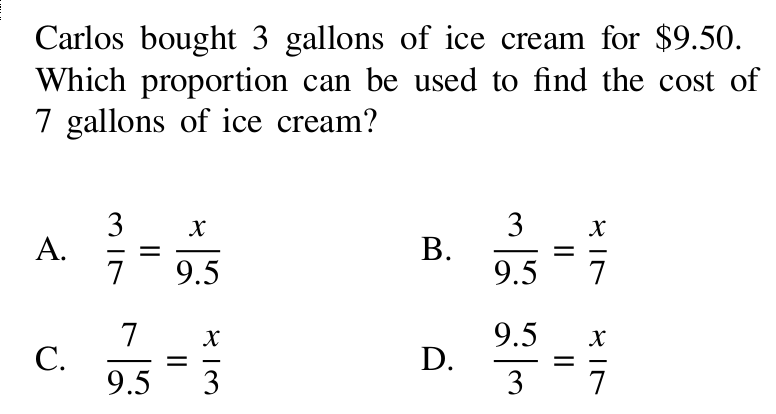
\includegraphics[width=0.8\linewidth]{EquivalentExpressionInContext1}

\leavevmode\\\relax 



\smallskip
\goodbreak
\hrule
\nobreak
\smallskip

%%% BEGIN PROBLEM PREAMBLE
{\bf 12.} (1 point) \ifdim\lastskip=\pgmlMarker
  \let\pgmlPar=\relax
 \else
  \let\pgmlPar=\par
  \vadjust{\kern3pt}%
\fi

%%%%%%%%%%%%%%%%%%%%%%%%%%%%%%%%%%%%%%
%
%    definitions for PGML
%

\ifx\pgmlCount\undefined  % do not redefine if multiple files load PGML.pl
  \newcount\pgmlCount
  \newdimen\pgmlPercent
  \newdimen\pgmlPixels  \pgmlPixels=.5pt
\fi
\pgmlPercent=.01\hsize

\def\pgmlSetup{%
  \parskip=0pt \parindent=0pt
%  \ifdim\lastskip=\pgmlMarker\else\par\fi
  \pgmlPar
}%

\def\pgmlIndent{\par\advance\leftskip by 2em \advance\pgmlPercent by .02em \pgmlCount=0}%
\def\pgmlbulletItem{\par\indent\llap{$\bullet$ }\ignorespaces}%
\def\pgmlcircleItem{\par\indent\llap{$\circ$ }\ignorespaces}%
\def\pgmlsquareItem{\par\indent\llap{\vrule height 1ex width .75ex depth -.25ex\ }\ignorespaces}%
\def\pgmlnumericItem{\par\indent\advance\pgmlCount by 1 \llap{\the\pgmlCount. }\ignorespaces}%
\def\pgmlalphaItem{\par\indent{\advance\pgmlCount by `\a \llap{\char\pgmlCount. }}\advance\pgmlCount by 1\ignorespaces}%
\def\pgmlAlphaItem{\par\indent{\advance\pgmlCount by `\A \llap{\char\pgmlCount. }}\advance\pgmlCount by 1\ignorespaces}%
\def\pgmlromanItem{\par\indent\advance\pgmlCount by 1 \llap{\romannumeral\pgmlCount. }\ignorespaces}%
\def\pgmlRomanItem{\par\indent\advance\pgmlCount by 1 \llap{\uppercase\expandafter{\romannumeral\pgmlCount}. }\ignorespaces}%

\def\pgmlCenter{%
  \par \parfillskip=0pt
  \advance\leftskip by 0pt plus .5\hsize
  \advance\rightskip by 0pt plus .5\hsize
  \def\pgmlBreak{\break}%
}%
\def\pgmlRight{%
  \par \parfillskip=0pt
  \advance\leftskip by 0pt plus \hsize
  \def\pgmlBreak{\break}%
}%

\def\pgmlBreak{\\}%

\def\pgmlHeading#1{%
  \par\bfseries
  \ifcase#1 \or\huge \or\LARGE \or\large \or\normalsize \or\footnotesize \or\scriptsize \fi
}%

\def\pgmlRule#1#2{%
  \par\noindent
  \hbox{%
    \strut%
    \dimen1=\ht\strutbox%
    \advance\dimen1 by -#2%
    \divide\dimen1 by 2%
    \advance\dimen2 by -\dp\strutbox%
    \raise\dimen1\hbox{\vrule width #1 height #2 depth 0pt}%
  }%
  \par
}%

\def\pgmlIC#1{\futurelet\pgmlNext\pgmlCheckIC}%
\def\pgmlCheckIC{\ifx\pgmlNext\pgmlSpace \/\fi}%
{\def\getSpace#1{\global\let\pgmlSpace= }\getSpace{} }%

{\catcode`\ =12\global\let\pgmlSpaceChar= }%
{\obeylines\gdef\pgmlPreformatted{\par\small\ttfamily\hsize=10\hsize\obeyspaces\obeylines\let^^M=\pgmlNL\pgmlNL}}%
\def\pgmlNL{\par\bgroup\catcode`\ =12\pgmlTestSpace}%
\def\pgmlTestSpace{\futurelet\next\pgmlTestChar}%
\def\pgmlTestChar{\ifx\next\pgmlSpaceChar\ \pgmlTestNext\fi\egroup}%
\def\pgmlTestNext\fi\egroup#1{\fi\pgmlTestSpace}%

\def^^M{\ifmmode\else\space\fi\ignorespaces}%
%%%%%%%%%%%%%%%%%%%%%%%%%%%%%%%%%%%%%%

%%% END PROBLEM PREAMBLE
Solve the following proportions: 
\smallskip
\par 
(a) \(\frac{15}{k} = \frac{6}{22}\)

\smallskip
\par 

k =  \mbox{\parbox[t]{12.5ex}{\hrulefill}}

\smallskip
\par 
(b) \(\frac{12}{25} = \frac{x}{88}\)

\smallskip
\par 
x =  \mbox{\parbox[t]{12.5ex}{\hrulefill}}


\smallskip
\goodbreak
\hrule
\nobreak
\smallskip

%%% BEGIN PROBLEM PREAMBLE
{\bf 13.} (1 point) \ifdim\lastskip=\pgmlMarker
  \let\pgmlPar=\relax
 \else
  \let\pgmlPar=\par
  \vadjust{\kern3pt}%
\fi

%%%%%%%%%%%%%%%%%%%%%%%%%%%%%%%%%%%%%%
%
%    definitions for PGML
%

\ifx\pgmlCount\undefined  % do not redefine if multiple files load PGML.pl
  \newcount\pgmlCount
  \newdimen\pgmlPercent
  \newdimen\pgmlPixels  \pgmlPixels=.5pt
\fi
\pgmlPercent=.01\hsize

\def\pgmlSetup{%
  \parskip=0pt \parindent=0pt
%  \ifdim\lastskip=\pgmlMarker\else\par\fi
  \pgmlPar
}%

\def\pgmlIndent{\par\advance\leftskip by 2em \advance\pgmlPercent by .02em \pgmlCount=0}%
\def\pgmlbulletItem{\par\indent\llap{$\bullet$ }\ignorespaces}%
\def\pgmlcircleItem{\par\indent\llap{$\circ$ }\ignorespaces}%
\def\pgmlsquareItem{\par\indent\llap{\vrule height 1ex width .75ex depth -.25ex\ }\ignorespaces}%
\def\pgmlnumericItem{\par\indent\advance\pgmlCount by 1 \llap{\the\pgmlCount. }\ignorespaces}%
\def\pgmlalphaItem{\par\indent{\advance\pgmlCount by `\a \llap{\char\pgmlCount. }}\advance\pgmlCount by 1\ignorespaces}%
\def\pgmlAlphaItem{\par\indent{\advance\pgmlCount by `\A \llap{\char\pgmlCount. }}\advance\pgmlCount by 1\ignorespaces}%
\def\pgmlromanItem{\par\indent\advance\pgmlCount by 1 \llap{\romannumeral\pgmlCount. }\ignorespaces}%
\def\pgmlRomanItem{\par\indent\advance\pgmlCount by 1 \llap{\uppercase\expandafter{\romannumeral\pgmlCount}. }\ignorespaces}%

\def\pgmlCenter{%
  \par \parfillskip=0pt
  \advance\leftskip by 0pt plus .5\hsize
  \advance\rightskip by 0pt plus .5\hsize
  \def\pgmlBreak{\break}%
}%
\def\pgmlRight{%
  \par \parfillskip=0pt
  \advance\leftskip by 0pt plus \hsize
  \def\pgmlBreak{\break}%
}%

\def\pgmlBreak{\\}%

\def\pgmlHeading#1{%
  \par\bfseries
  \ifcase#1 \or\huge \or\LARGE \or\large \or\normalsize \or\footnotesize \or\scriptsize \fi
}%

\def\pgmlRule#1#2{%
  \par\noindent
  \hbox{%
    \strut%
    \dimen1=\ht\strutbox%
    \advance\dimen1 by -#2%
    \divide\dimen1 by 2%
    \advance\dimen2 by -\dp\strutbox%
    \raise\dimen1\hbox{\vrule width #1 height #2 depth 0pt}%
  }%
  \par
}%

\def\pgmlIC#1{\futurelet\pgmlNext\pgmlCheckIC}%
\def\pgmlCheckIC{\ifx\pgmlNext\pgmlSpace \/\fi}%
{\def\getSpace#1{\global\let\pgmlSpace= }\getSpace{} }%

{\catcode`\ =12\global\let\pgmlSpaceChar= }%
{\obeylines\gdef\pgmlPreformatted{\par\small\ttfamily\hsize=10\hsize\obeyspaces\obeylines\let^^M=\pgmlNL\pgmlNL}}%
\def\pgmlNL{\par\bgroup\catcode`\ =12\pgmlTestSpace}%
\def\pgmlTestSpace{\futurelet\next\pgmlTestChar}%
\def\pgmlTestChar{\ifx\next\pgmlSpaceChar\ \pgmlTestNext\fi\egroup}%
\def\pgmlTestNext\fi\egroup#1{\fi\pgmlTestSpace}%

\def^^M{\ifmmode\else\space\fi\ignorespaces}%
%%%%%%%%%%%%%%%%%%%%%%%%%%%%%%%%%%%%%%

%%% END PROBLEM PREAMBLE
Simplify

\smallskip
\par 
\(-2 b +(7 b -3)\)=  \mbox{\parbox[t]{25ex}{\hrulefill}}



\smallskip
\goodbreak
\hrule
\nobreak
\smallskip

    \ifx\pgmlMarker\undefined
      \newdimen\pgmlMarker \pgmlMarker=0.00314159pt  % hack to tell if \newline was used
    \fi
    \ifx\oldnewline\undefined \let\oldnewline=\newline \fi
    \def\newline{\oldnewline\hskip-\pgmlMarker\hskip\pgmlMarker\relax}%
    \parindent=0pt
    \catcode`\^^M=\active
    \def^^M{\ifmmode\else\fi\ignorespaces}%  skip paragraph breaks in the preamble
    \def\par{\ifmmode\else\endgraf\fi\ignorespaces}%
  
%%% BEGIN PROBLEM PREAMBLE
{\bf 14.} (1 point) \ifdim\lastskip=\pgmlMarker
  \let\pgmlPar=\relax
 \else
  \let\pgmlPar=\par
  \vadjust{\kern3pt}%
\fi

%%%%%%%%%%%%%%%%%%%%%%%%%%%%%%%%%%%%%%
%
%    definitions for PGML
%

\ifx\pgmlCount\undefined  % do not redefine if multiple files load PGML.pl
  \newcount\pgmlCount
  \newdimen\pgmlPercent
  \newdimen\pgmlPixels  \pgmlPixels=.5pt
\fi
\pgmlPercent=.01\hsize

\def\pgmlSetup{%
  \parskip=0pt \parindent=0pt
%  \ifdim\lastskip=\pgmlMarker\else\par\fi
  \pgmlPar
}%

\def\pgmlIndent{\par\advance\leftskip by 2em \advance\pgmlPercent by .02em \pgmlCount=0}%
\def\pgmlbulletItem{\par\indent\llap{$\bullet$ }\ignorespaces}%
\def\pgmlcircleItem{\par\indent\llap{$\circ$ }\ignorespaces}%
\def\pgmlsquareItem{\par\indent\llap{\vrule height 1ex width .75ex depth -.25ex\ }\ignorespaces}%
\def\pgmlnumericItem{\par\indent\advance\pgmlCount by 1 \llap{\the\pgmlCount. }\ignorespaces}%
\def\pgmlalphaItem{\par\indent{\advance\pgmlCount by `\a \llap{\char\pgmlCount. }}\advance\pgmlCount by 1\ignorespaces}%
\def\pgmlAlphaItem{\par\indent{\advance\pgmlCount by `\A \llap{\char\pgmlCount. }}\advance\pgmlCount by 1\ignorespaces}%
\def\pgmlromanItem{\par\indent\advance\pgmlCount by 1 \llap{\romannumeral\pgmlCount. }\ignorespaces}%
\def\pgmlRomanItem{\par\indent\advance\pgmlCount by 1 \llap{\uppercase\expandafter{\romannumeral\pgmlCount}. }\ignorespaces}%

\def\pgmlCenter{%
  \par \parfillskip=0pt
  \advance\leftskip by 0pt plus .5\hsize
  \advance\rightskip by 0pt plus .5\hsize
  \def\pgmlBreak{\break}%
}%
\def\pgmlRight{%
  \par \parfillskip=0pt
  \advance\leftskip by 0pt plus \hsize
  \def\pgmlBreak{\break}%
}%

\def\pgmlBreak{\\}%

\def\pgmlHeading#1{%
  \par\bfseries
  \ifcase#1 \or\huge \or\LARGE \or\large \or\normalsize \or\footnotesize \or\scriptsize \fi
}%

\def\pgmlRule#1#2{%
  \par\noindent
  \hbox{%
    \strut%
    \dimen1=\ht\strutbox%
    \advance\dimen1 by -#2%
    \divide\dimen1 by 2%
    \advance\dimen2 by -\dp\strutbox%
    \raise\dimen1\hbox{\vrule width #1 height #2 depth 0pt}%
  }%
  \par
}%

\def\pgmlIC#1{\futurelet\pgmlNext\pgmlCheckIC}%
\def\pgmlCheckIC{\ifx\pgmlNext\pgmlSpace \/\fi}%
{\def\getSpace#1{\global\let\pgmlSpace= }\getSpace{} }%

{\catcode`\ =12\global\let\pgmlSpaceChar= }%
{\obeylines\gdef\pgmlPreformatted{\par\small\ttfamily\hsize=10\hsize\obeyspaces\obeylines\let^^M=\pgmlNL\pgmlNL}}%
\def\pgmlNL{\par\bgroup\catcode`\ =12\pgmlTestSpace}%
\def\pgmlTestSpace{\futurelet\next\pgmlTestChar}%
\def\pgmlTestChar{\ifx\next\pgmlSpaceChar\ \pgmlTestNext\fi\egroup}%
\def\pgmlTestNext\fi\egroup#1{\fi\pgmlTestSpace}%

\def^^M{\ifmmode\else\space\fi\ignorespaces}%
%%%%%%%%%%%%%%%%%%%%%%%%%%%%%%%%%%%%%%

%%% END PROBLEM PREAMBLE

Here are three stacks of coins. Stack A has
20 coins, stack B has 13 coins, and stack C has
19 coins.

\leavevmode\\\relax 
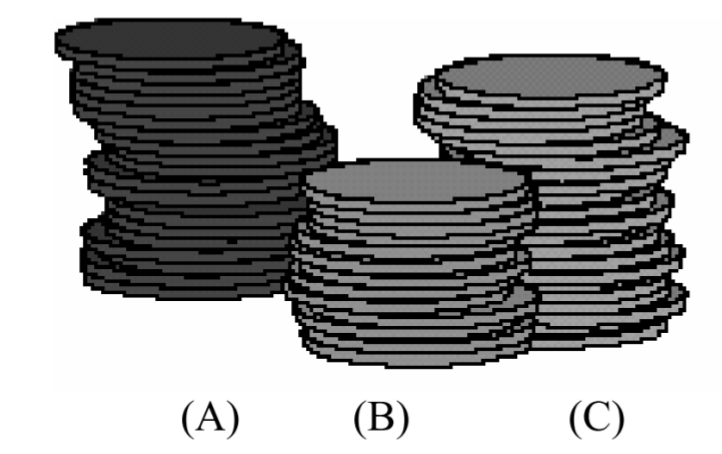
\includegraphics[width=0.8\linewidth]{Percent1}

\leavevmode\\\relax 
What percent of the total coins is in Stack B?
\leavevmode\\\relax 

\medskip
\par
 \mbox{\parbox[t]{12.5ex}{\hrulefill}}



\smallskip
\goodbreak
\hrule
\nobreak
\smallskip

    \ifx\pgmlMarker\undefined
      \newdimen\pgmlMarker \pgmlMarker=0.00314159pt  % hack to tell if \newline was used
    \fi
    \ifx\oldnewline\undefined \let\oldnewline=\newline \fi
    \def\newline{\oldnewline\hskip-\pgmlMarker\hskip\pgmlMarker\relax}%
    \parindent=0pt
    \catcode`\^^M=\active
    \def^^M{\ifmmode\else\fi\ignorespaces}%  skip paragraph breaks in the preamble
    \def\par{\ifmmode\else\endgraf\fi\ignorespaces}%
  
%%% BEGIN PROBLEM PREAMBLE
{\bf 15.} (1 point) \ifdim\lastskip=\pgmlMarker
  \let\pgmlPar=\relax
 \else
  \let\pgmlPar=\par
  \vadjust{\kern3pt}%
\fi

%%%%%%%%%%%%%%%%%%%%%%%%%%%%%%%%%%%%%%
%
%    definitions for PGML
%

\ifx\pgmlCount\undefined  % do not redefine if multiple files load PGML.pl
  \newcount\pgmlCount
  \newdimen\pgmlPercent
  \newdimen\pgmlPixels  \pgmlPixels=.5pt
\fi
\pgmlPercent=.01\hsize

\def\pgmlSetup{%
  \parskip=0pt \parindent=0pt
%  \ifdim\lastskip=\pgmlMarker\else\par\fi
  \pgmlPar
}%

\def\pgmlIndent{\par\advance\leftskip by 2em \advance\pgmlPercent by .02em \pgmlCount=0}%
\def\pgmlbulletItem{\par\indent\llap{$\bullet$ }\ignorespaces}%
\def\pgmlcircleItem{\par\indent\llap{$\circ$ }\ignorespaces}%
\def\pgmlsquareItem{\par\indent\llap{\vrule height 1ex width .75ex depth -.25ex\ }\ignorespaces}%
\def\pgmlnumericItem{\par\indent\advance\pgmlCount by 1 \llap{\the\pgmlCount. }\ignorespaces}%
\def\pgmlalphaItem{\par\indent{\advance\pgmlCount by `\a \llap{\char\pgmlCount. }}\advance\pgmlCount by 1\ignorespaces}%
\def\pgmlAlphaItem{\par\indent{\advance\pgmlCount by `\A \llap{\char\pgmlCount. }}\advance\pgmlCount by 1\ignorespaces}%
\def\pgmlromanItem{\par\indent\advance\pgmlCount by 1 \llap{\romannumeral\pgmlCount. }\ignorespaces}%
\def\pgmlRomanItem{\par\indent\advance\pgmlCount by 1 \llap{\uppercase\expandafter{\romannumeral\pgmlCount}. }\ignorespaces}%

\def\pgmlCenter{%
  \par \parfillskip=0pt
  \advance\leftskip by 0pt plus .5\hsize
  \advance\rightskip by 0pt plus .5\hsize
  \def\pgmlBreak{\break}%
}%
\def\pgmlRight{%
  \par \parfillskip=0pt
  \advance\leftskip by 0pt plus \hsize
  \def\pgmlBreak{\break}%
}%

\def\pgmlBreak{\\}%

\def\pgmlHeading#1{%
  \par\bfseries
  \ifcase#1 \or\huge \or\LARGE \or\large \or\normalsize \or\footnotesize \or\scriptsize \fi
}%

\def\pgmlRule#1#2{%
  \par\noindent
  \hbox{%
    \strut%
    \dimen1=\ht\strutbox%
    \advance\dimen1 by -#2%
    \divide\dimen1 by 2%
    \advance\dimen2 by -\dp\strutbox%
    \raise\dimen1\hbox{\vrule width #1 height #2 depth 0pt}%
  }%
  \par
}%

\def\pgmlIC#1{\futurelet\pgmlNext\pgmlCheckIC}%
\def\pgmlCheckIC{\ifx\pgmlNext\pgmlSpace \/\fi}%
{\def\getSpace#1{\global\let\pgmlSpace= }\getSpace{} }%

{\catcode`\ =12\global\let\pgmlSpaceChar= }%
{\obeylines\gdef\pgmlPreformatted{\par\small\ttfamily\hsize=10\hsize\obeyspaces\obeylines\let^^M=\pgmlNL\pgmlNL}}%
\def\pgmlNL{\par\bgroup\catcode`\ =12\pgmlTestSpace}%
\def\pgmlTestSpace{\futurelet\next\pgmlTestChar}%
\def\pgmlTestChar{\ifx\next\pgmlSpaceChar\ \pgmlTestNext\fi\egroup}%
\def\pgmlTestNext\fi\egroup#1{\fi\pgmlTestSpace}%

\def^^M{\ifmmode\else\space\fi\ignorespaces}%
%%%%%%%%%%%%%%%%%%%%%%%%%%%%%%%%%%%%%%

%%% END PROBLEM PREAMBLE

A baseball team won 75\% of its games. If the
team played 48 games, how many games did it
win?

\smallskip
\leavevmode\\\relax 

 \mbox{\parbox[t]{12.5ex}{\hrulefill}}



\smallskip
\goodbreak
\hrule
\nobreak
\smallskip

    \ifx\pgmlMarker\undefined
      \newdimen\pgmlMarker \pgmlMarker=0.00314159pt  % hack to tell if \newline was used
    \fi
    \ifx\oldnewline\undefined \let\oldnewline=\newline \fi
    \def\newline{\oldnewline\hskip-\pgmlMarker\hskip\pgmlMarker\relax}%
    \parindent=0pt
    \catcode`\^^M=\active
    \def^^M{\ifmmode\else\fi\ignorespaces}%  skip paragraph breaks in the preamble
    \def\par{\ifmmode\else\endgraf\fi\ignorespaces}%
  
%%% BEGIN PROBLEM PREAMBLE
{\bf 16.} (1 point) \ifdim\lastskip=\pgmlMarker
  \let\pgmlPar=\relax
 \else
  \let\pgmlPar=\par
  \vadjust{\kern3pt}%
\fi

%%%%%%%%%%%%%%%%%%%%%%%%%%%%%%%%%%%%%%
%
%    definitions for PGML
%

\ifx\pgmlCount\undefined  % do not redefine if multiple files load PGML.pl
  \newcount\pgmlCount
  \newdimen\pgmlPercent
  \newdimen\pgmlPixels  \pgmlPixels=.5pt
\fi
\pgmlPercent=.01\hsize

\def\pgmlSetup{%
  \parskip=0pt \parindent=0pt
%  \ifdim\lastskip=\pgmlMarker\else\par\fi
  \pgmlPar
}%

\def\pgmlIndent{\par\advance\leftskip by 2em \advance\pgmlPercent by .02em \pgmlCount=0}%
\def\pgmlbulletItem{\par\indent\llap{$\bullet$ }\ignorespaces}%
\def\pgmlcircleItem{\par\indent\llap{$\circ$ }\ignorespaces}%
\def\pgmlsquareItem{\par\indent\llap{\vrule height 1ex width .75ex depth -.25ex\ }\ignorespaces}%
\def\pgmlnumericItem{\par\indent\advance\pgmlCount by 1 \llap{\the\pgmlCount. }\ignorespaces}%
\def\pgmlalphaItem{\par\indent{\advance\pgmlCount by `\a \llap{\char\pgmlCount. }}\advance\pgmlCount by 1\ignorespaces}%
\def\pgmlAlphaItem{\par\indent{\advance\pgmlCount by `\A \llap{\char\pgmlCount. }}\advance\pgmlCount by 1\ignorespaces}%
\def\pgmlromanItem{\par\indent\advance\pgmlCount by 1 \llap{\romannumeral\pgmlCount. }\ignorespaces}%
\def\pgmlRomanItem{\par\indent\advance\pgmlCount by 1 \llap{\uppercase\expandafter{\romannumeral\pgmlCount}. }\ignorespaces}%

\def\pgmlCenter{%
  \par \parfillskip=0pt
  \advance\leftskip by 0pt plus .5\hsize
  \advance\rightskip by 0pt plus .5\hsize
  \def\pgmlBreak{\break}%
}%
\def\pgmlRight{%
  \par \parfillskip=0pt
  \advance\leftskip by 0pt plus \hsize
  \def\pgmlBreak{\break}%
}%

\def\pgmlBreak{\\}%

\def\pgmlHeading#1{%
  \par\bfseries
  \ifcase#1 \or\huge \or\LARGE \or\large \or\normalsize \or\footnotesize \or\scriptsize \fi
}%

\def\pgmlRule#1#2{%
  \par\noindent
  \hbox{%
    \strut%
    \dimen1=\ht\strutbox%
    \advance\dimen1 by -#2%
    \divide\dimen1 by 2%
    \advance\dimen2 by -\dp\strutbox%
    \raise\dimen1\hbox{\vrule width #1 height #2 depth 0pt}%
  }%
  \par
}%

\def\pgmlIC#1{\futurelet\pgmlNext\pgmlCheckIC}%
\def\pgmlCheckIC{\ifx\pgmlNext\pgmlSpace \/\fi}%
{\def\getSpace#1{\global\let\pgmlSpace= }\getSpace{} }%

{\catcode`\ =12\global\let\pgmlSpaceChar= }%
{\obeylines\gdef\pgmlPreformatted{\par\small\ttfamily\hsize=10\hsize\obeyspaces\obeylines\let^^M=\pgmlNL\pgmlNL}}%
\def\pgmlNL{\par\bgroup\catcode`\ =12\pgmlTestSpace}%
\def\pgmlTestSpace{\futurelet\next\pgmlTestChar}%
\def\pgmlTestChar{\ifx\next\pgmlSpaceChar\ \pgmlTestNext\fi\egroup}%
\def\pgmlTestNext\fi\egroup#1{\fi\pgmlTestSpace}%

\def^^M{\ifmmode\else\space\fi\ignorespaces}%
%%%%%%%%%%%%%%%%%%%%%%%%%%%%%%%%%%%%%%

%%% END PROBLEM PREAMBLE
{\pgmlSetup
Fill in the blanks with percent. Don't use calculator or paper/pencil. Use mental math.
\vskip\baselineskip
{\pgmlIndent\let\pgmlItem=\pgmlalphaItem
\smallskip
\pgmlItem{}\(20\) is   \mbox{\parbox[t]{25ex}{\hrulefill}} of \(10\)?

\smallskip
\pgmlItem{}\(6\) is   \mbox{\parbox[t]{25ex}{\hrulefill}} of \(2\)?
\par}%
\vskip\baselineskip
\par}%

\smallskip
\goodbreak
\hrule
\nobreak
\smallskip

    \ifx\pgmlMarker\undefined
      \newdimen\pgmlMarker \pgmlMarker=0.00314159pt  % hack to tell if \newline was used
    \fi
    \ifx\oldnewline\undefined \let\oldnewline=\newline \fi
    \def\newline{\oldnewline\hskip-\pgmlMarker\hskip\pgmlMarker\relax}%
    \parindent=0pt
    \catcode`\^^M=\active
    \def^^M{\ifmmode\else\fi\ignorespaces}%  skip paragraph breaks in the preamble
    \def\par{\ifmmode\else\endgraf\fi\ignorespaces}%
  
%%% BEGIN PROBLEM PREAMBLE
{\bf 17.} (1 point) \ifdim\lastskip=\pgmlMarker
  \let\pgmlPar=\relax
 \else
  \let\pgmlPar=\par
  \vadjust{\kern3pt}%
\fi

%%%%%%%%%%%%%%%%%%%%%%%%%%%%%%%%%%%%%%
%
%    definitions for PGML
%

\ifx\pgmlCount\undefined  % do not redefine if multiple files load PGML.pl
  \newcount\pgmlCount
  \newdimen\pgmlPercent
  \newdimen\pgmlPixels  \pgmlPixels=.5pt
\fi
\pgmlPercent=.01\hsize

\def\pgmlSetup{%
  \parskip=0pt \parindent=0pt
%  \ifdim\lastskip=\pgmlMarker\else\par\fi
  \pgmlPar
}%

\def\pgmlIndent{\par\advance\leftskip by 2em \advance\pgmlPercent by .02em \pgmlCount=0}%
\def\pgmlbulletItem{\par\indent\llap{$\bullet$ }\ignorespaces}%
\def\pgmlcircleItem{\par\indent\llap{$\circ$ }\ignorespaces}%
\def\pgmlsquareItem{\par\indent\llap{\vrule height 1ex width .75ex depth -.25ex\ }\ignorespaces}%
\def\pgmlnumericItem{\par\indent\advance\pgmlCount by 1 \llap{\the\pgmlCount. }\ignorespaces}%
\def\pgmlalphaItem{\par\indent{\advance\pgmlCount by `\a \llap{\char\pgmlCount. }}\advance\pgmlCount by 1\ignorespaces}%
\def\pgmlAlphaItem{\par\indent{\advance\pgmlCount by `\A \llap{\char\pgmlCount. }}\advance\pgmlCount by 1\ignorespaces}%
\def\pgmlromanItem{\par\indent\advance\pgmlCount by 1 \llap{\romannumeral\pgmlCount. }\ignorespaces}%
\def\pgmlRomanItem{\par\indent\advance\pgmlCount by 1 \llap{\uppercase\expandafter{\romannumeral\pgmlCount}. }\ignorespaces}%

\def\pgmlCenter{%
  \par \parfillskip=0pt
  \advance\leftskip by 0pt plus .5\hsize
  \advance\rightskip by 0pt plus .5\hsize
  \def\pgmlBreak{\break}%
}%
\def\pgmlRight{%
  \par \parfillskip=0pt
  \advance\leftskip by 0pt plus \hsize
  \def\pgmlBreak{\break}%
}%

\def\pgmlBreak{\\}%

\def\pgmlHeading#1{%
  \par\bfseries
  \ifcase#1 \or\huge \or\LARGE \or\large \or\normalsize \or\footnotesize \or\scriptsize \fi
}%

\def\pgmlRule#1#2{%
  \par\noindent
  \hbox{%
    \strut%
    \dimen1=\ht\strutbox%
    \advance\dimen1 by -#2%
    \divide\dimen1 by 2%
    \advance\dimen2 by -\dp\strutbox%
    \raise\dimen1\hbox{\vrule width #1 height #2 depth 0pt}%
  }%
  \par
}%

\def\pgmlIC#1{\futurelet\pgmlNext\pgmlCheckIC}%
\def\pgmlCheckIC{\ifx\pgmlNext\pgmlSpace \/\fi}%
{\def\getSpace#1{\global\let\pgmlSpace= }\getSpace{} }%

{\catcode`\ =12\global\let\pgmlSpaceChar= }%
{\obeylines\gdef\pgmlPreformatted{\par\small\ttfamily\hsize=10\hsize\obeyspaces\obeylines\let^^M=\pgmlNL\pgmlNL}}%
\def\pgmlNL{\par\bgroup\catcode`\ =12\pgmlTestSpace}%
\def\pgmlTestSpace{\futurelet\next\pgmlTestChar}%
\def\pgmlTestChar{\ifx\next\pgmlSpaceChar\ \pgmlTestNext\fi\egroup}%
\def\pgmlTestNext\fi\egroup#1{\fi\pgmlTestSpace}%

\def^^M{\ifmmode\else\space\fi\ignorespaces}%
%%%%%%%%%%%%%%%%%%%%%%%%%%%%%%%%%%%%%%

%%% END PROBLEM PREAMBLE

The shaded area of the picture below shows
what part of the yard Jessie mowed in
30 minutes.

\leavevmode\\\relax 
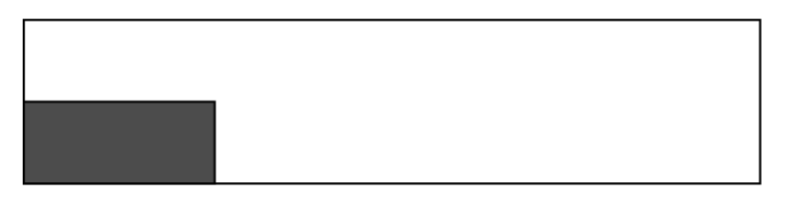
\includegraphics[width=0.8\linewidth]{ProportionalRelationships3}

\leavevmode\\\relax 
She wonders about how long it takes her to mow
the WHOLE yard. Write a note to Jessie
\leavevmode\\\relax 
A. telling her about how long it takes to mow her WHOLE yard, and 
\leavevmode\\\relax 
B. explaining to her how you found your answer.

\vskip 2.56 in \hrulefill\quad 



\smallskip
\goodbreak
\hrule
\nobreak
\smallskip

%%% BEGIN PROBLEM PREAMBLE
{\bf 18.} (1 point) \ifdim\lastskip=\pgmlMarker
  \let\pgmlPar=\relax
 \else
  \let\pgmlPar=\par
  \vadjust{\kern3pt}%
\fi

%%%%%%%%%%%%%%%%%%%%%%%%%%%%%%%%%%%%%%
%
%    definitions for PGML
%

\ifx\pgmlCount\undefined  % do not redefine if multiple files load PGML.pl
  \newcount\pgmlCount
  \newdimen\pgmlPercent
  \newdimen\pgmlPixels  \pgmlPixels=.5pt
\fi
\pgmlPercent=.01\hsize

\def\pgmlSetup{%
  \parskip=0pt \parindent=0pt
%  \ifdim\lastskip=\pgmlMarker\else\par\fi
  \pgmlPar
}%

\def\pgmlIndent{\par\advance\leftskip by 2em \advance\pgmlPercent by .02em \pgmlCount=0}%
\def\pgmlbulletItem{\par\indent\llap{$\bullet$ }\ignorespaces}%
\def\pgmlcircleItem{\par\indent\llap{$\circ$ }\ignorespaces}%
\def\pgmlsquareItem{\par\indent\llap{\vrule height 1ex width .75ex depth -.25ex\ }\ignorespaces}%
\def\pgmlnumericItem{\par\indent\advance\pgmlCount by 1 \llap{\the\pgmlCount. }\ignorespaces}%
\def\pgmlalphaItem{\par\indent{\advance\pgmlCount by `\a \llap{\char\pgmlCount. }}\advance\pgmlCount by 1\ignorespaces}%
\def\pgmlAlphaItem{\par\indent{\advance\pgmlCount by `\A \llap{\char\pgmlCount. }}\advance\pgmlCount by 1\ignorespaces}%
\def\pgmlromanItem{\par\indent\advance\pgmlCount by 1 \llap{\romannumeral\pgmlCount. }\ignorespaces}%
\def\pgmlRomanItem{\par\indent\advance\pgmlCount by 1 \llap{\uppercase\expandafter{\romannumeral\pgmlCount}. }\ignorespaces}%

\def\pgmlCenter{%
  \par \parfillskip=0pt
  \advance\leftskip by 0pt plus .5\hsize
  \advance\rightskip by 0pt plus .5\hsize
  \def\pgmlBreak{\break}%
}%
\def\pgmlRight{%
  \par \parfillskip=0pt
  \advance\leftskip by 0pt plus \hsize
  \def\pgmlBreak{\break}%
}%

\def\pgmlBreak{\\}%

\def\pgmlHeading#1{%
  \par\bfseries
  \ifcase#1 \or\huge \or\LARGE \or\large \or\normalsize \or\footnotesize \or\scriptsize \fi
}%

\def\pgmlRule#1#2{%
  \par\noindent
  \hbox{%
    \strut%
    \dimen1=\ht\strutbox%
    \advance\dimen1 by -#2%
    \divide\dimen1 by 2%
    \advance\dimen2 by -\dp\strutbox%
    \raise\dimen1\hbox{\vrule width #1 height #2 depth 0pt}%
  }%
  \par
}%

\def\pgmlIC#1{\futurelet\pgmlNext\pgmlCheckIC}%
\def\pgmlCheckIC{\ifx\pgmlNext\pgmlSpace \/\fi}%
{\def\getSpace#1{\global\let\pgmlSpace= }\getSpace{} }%

{\catcode`\ =12\global\let\pgmlSpaceChar= }%
{\obeylines\gdef\pgmlPreformatted{\par\small\ttfamily\hsize=10\hsize\obeyspaces\obeylines\let^^M=\pgmlNL\pgmlNL}}%
\def\pgmlNL{\par\bgroup\catcode`\ =12\pgmlTestSpace}%
\def\pgmlTestSpace{\futurelet\next\pgmlTestChar}%
\def\pgmlTestChar{\ifx\next\pgmlSpaceChar\ \pgmlTestNext\fi\egroup}%
\def\pgmlTestNext\fi\egroup#1{\fi\pgmlTestSpace}%

\def^^M{\ifmmode\else\space\fi\ignorespaces}%
%%%%%%%%%%%%%%%%%%%%%%%%%%%%%%%%%%%%%%

%%% END PROBLEM PREAMBLE
Evaluate: \(7 \cdot 3 - 2 \cdot 2^2 + 5 (9 - 3)\)
\vspace{0.25cm}
\par 
Answer:   \mbox{\parbox[t]{25ex}{\hrulefill}}

  \leavevmode\\\relax 

\smallskip
\goodbreak
\hrule
\nobreak
\smallskip

%%% BEGIN PROBLEM PREAMBLE
{\bf 19.} (1 point) \ifdim\lastskip=\pgmlMarker
  \let\pgmlPar=\relax
 \else
  \let\pgmlPar=\par
  \vadjust{\kern3pt}%
\fi

%%%%%%%%%%%%%%%%%%%%%%%%%%%%%%%%%%%%%%
%
%    definitions for PGML
%

\ifx\pgmlCount\undefined  % do not redefine if multiple files load PGML.pl
  \newcount\pgmlCount
  \newdimen\pgmlPercent
  \newdimen\pgmlPixels  \pgmlPixels=.5pt
\fi
\pgmlPercent=.01\hsize

\def\pgmlSetup{%
  \parskip=0pt \parindent=0pt
%  \ifdim\lastskip=\pgmlMarker\else\par\fi
  \pgmlPar
}%

\def\pgmlIndent{\par\advance\leftskip by 2em \advance\pgmlPercent by .02em \pgmlCount=0}%
\def\pgmlbulletItem{\par\indent\llap{$\bullet$ }\ignorespaces}%
\def\pgmlcircleItem{\par\indent\llap{$\circ$ }\ignorespaces}%
\def\pgmlsquareItem{\par\indent\llap{\vrule height 1ex width .75ex depth -.25ex\ }\ignorespaces}%
\def\pgmlnumericItem{\par\indent\advance\pgmlCount by 1 \llap{\the\pgmlCount. }\ignorespaces}%
\def\pgmlalphaItem{\par\indent{\advance\pgmlCount by `\a \llap{\char\pgmlCount. }}\advance\pgmlCount by 1\ignorespaces}%
\def\pgmlAlphaItem{\par\indent{\advance\pgmlCount by `\A \llap{\char\pgmlCount. }}\advance\pgmlCount by 1\ignorespaces}%
\def\pgmlromanItem{\par\indent\advance\pgmlCount by 1 \llap{\romannumeral\pgmlCount. }\ignorespaces}%
\def\pgmlRomanItem{\par\indent\advance\pgmlCount by 1 \llap{\uppercase\expandafter{\romannumeral\pgmlCount}. }\ignorespaces}%

\def\pgmlCenter{%
  \par \parfillskip=0pt
  \advance\leftskip by 0pt plus .5\hsize
  \advance\rightskip by 0pt plus .5\hsize
  \def\pgmlBreak{\break}%
}%
\def\pgmlRight{%
  \par \parfillskip=0pt
  \advance\leftskip by 0pt plus \hsize
  \def\pgmlBreak{\break}%
}%

\def\pgmlBreak{\\}%

\def\pgmlHeading#1{%
  \par\bfseries
  \ifcase#1 \or\huge \or\LARGE \or\large \or\normalsize \or\footnotesize \or\scriptsize \fi
}%

\def\pgmlRule#1#2{%
  \par\noindent
  \hbox{%
    \strut%
    \dimen1=\ht\strutbox%
    \advance\dimen1 by -#2%
    \divide\dimen1 by 2%
    \advance\dimen2 by -\dp\strutbox%
    \raise\dimen1\hbox{\vrule width #1 height #2 depth 0pt}%
  }%
  \par
}%

\def\pgmlIC#1{\futurelet\pgmlNext\pgmlCheckIC}%
\def\pgmlCheckIC{\ifx\pgmlNext\pgmlSpace \/\fi}%
{\def\getSpace#1{\global\let\pgmlSpace= }\getSpace{} }%

{\catcode`\ =12\global\let\pgmlSpaceChar= }%
{\obeylines\gdef\pgmlPreformatted{\par\small\ttfamily\hsize=10\hsize\obeyspaces\obeylines\let^^M=\pgmlNL\pgmlNL}}%
\def\pgmlNL{\par\bgroup\catcode`\ =12\pgmlTestSpace}%
\def\pgmlTestSpace{\futurelet\next\pgmlTestChar}%
\def\pgmlTestChar{\ifx\next\pgmlSpaceChar\ \pgmlTestNext\fi\egroup}%
\def\pgmlTestNext\fi\egroup#1{\fi\pgmlTestSpace}%

\def^^M{\ifmmode\else\space\fi\ignorespaces}%
%%%%%%%%%%%%%%%%%%%%%%%%%%%%%%%%%%%%%%

%%% END PROBLEM PREAMBLE
Simplify

\vspace{0.25cm}
\par 
\(2 b -(9 b -2)\)=    \mbox{\parbox[t]{25ex}{\hrulefill}}



\smallskip
\goodbreak
\hrule
\nobreak
\smallskip

%%% BEGIN PROBLEM PREAMBLE
{\bf 20.} (1 point) \ifdim\lastskip=\pgmlMarker
  \let\pgmlPar=\relax
 \else
  \let\pgmlPar=\par
  \vadjust{\kern3pt}%
\fi

%%%%%%%%%%%%%%%%%%%%%%%%%%%%%%%%%%%%%%
%
%    definitions for PGML
%

\ifx\pgmlCount\undefined  % do not redefine if multiple files load PGML.pl
  \newcount\pgmlCount
  \newdimen\pgmlPercent
  \newdimen\pgmlPixels  \pgmlPixels=.5pt
\fi
\pgmlPercent=.01\hsize

\def\pgmlSetup{%
  \parskip=0pt \parindent=0pt
%  \ifdim\lastskip=\pgmlMarker\else\par\fi
  \pgmlPar
}%

\def\pgmlIndent{\par\advance\leftskip by 2em \advance\pgmlPercent by .02em \pgmlCount=0}%
\def\pgmlbulletItem{\par\indent\llap{$\bullet$ }\ignorespaces}%
\def\pgmlcircleItem{\par\indent\llap{$\circ$ }\ignorespaces}%
\def\pgmlsquareItem{\par\indent\llap{\vrule height 1ex width .75ex depth -.25ex\ }\ignorespaces}%
\def\pgmlnumericItem{\par\indent\advance\pgmlCount by 1 \llap{\the\pgmlCount. }\ignorespaces}%
\def\pgmlalphaItem{\par\indent{\advance\pgmlCount by `\a \llap{\char\pgmlCount. }}\advance\pgmlCount by 1\ignorespaces}%
\def\pgmlAlphaItem{\par\indent{\advance\pgmlCount by `\A \llap{\char\pgmlCount. }}\advance\pgmlCount by 1\ignorespaces}%
\def\pgmlromanItem{\par\indent\advance\pgmlCount by 1 \llap{\romannumeral\pgmlCount. }\ignorespaces}%
\def\pgmlRomanItem{\par\indent\advance\pgmlCount by 1 \llap{\uppercase\expandafter{\romannumeral\pgmlCount}. }\ignorespaces}%

\def\pgmlCenter{%
  \par \parfillskip=0pt
  \advance\leftskip by 0pt plus .5\hsize
  \advance\rightskip by 0pt plus .5\hsize
  \def\pgmlBreak{\break}%
}%
\def\pgmlRight{%
  \par \parfillskip=0pt
  \advance\leftskip by 0pt plus \hsize
  \def\pgmlBreak{\break}%
}%

\def\pgmlBreak{\\}%

\def\pgmlHeading#1{%
  \par\bfseries
  \ifcase#1 \or\huge \or\LARGE \or\large \or\normalsize \or\footnotesize \or\scriptsize \fi
}%

\def\pgmlRule#1#2{%
  \par\noindent
  \hbox{%
    \strut%
    \dimen1=\ht\strutbox%
    \advance\dimen1 by -#2%
    \divide\dimen1 by 2%
    \advance\dimen2 by -\dp\strutbox%
    \raise\dimen1\hbox{\vrule width #1 height #2 depth 0pt}%
  }%
  \par
}%

\def\pgmlIC#1{\futurelet\pgmlNext\pgmlCheckIC}%
\def\pgmlCheckIC{\ifx\pgmlNext\pgmlSpace \/\fi}%
{\def\getSpace#1{\global\let\pgmlSpace= }\getSpace{} }%

{\catcode`\ =12\global\let\pgmlSpaceChar= }%
{\obeylines\gdef\pgmlPreformatted{\par\small\ttfamily\hsize=10\hsize\obeyspaces\obeylines\let^^M=\pgmlNL\pgmlNL}}%
\def\pgmlNL{\par\bgroup\catcode`\ =12\pgmlTestSpace}%
\def\pgmlTestSpace{\futurelet\next\pgmlTestChar}%
\def\pgmlTestChar{\ifx\next\pgmlSpaceChar\ \pgmlTestNext\fi\egroup}%
\def\pgmlTestNext\fi\egroup#1{\fi\pgmlTestSpace}%

\def^^M{\ifmmode\else\space\fi\ignorespaces}%
%%%%%%%%%%%%%%%%%%%%%%%%%%%%%%%%%%%%%%

%%% END PROBLEM PREAMBLE
Simplify

\vspace{0.25cm}
\par 
\(4 b -(7 b +2)\)=  \mbox{\parbox[t]{25ex}{\hrulefill}}



\smallskip
\goodbreak
\hrule
\nobreak
\smallskip

%%% BEGIN PROBLEM PREAMBLE
{\bf 21.} (1 point) \ifdim\lastskip=\pgmlMarker
  \let\pgmlPar=\relax
 \else
  \let\pgmlPar=\par
  \vadjust{\kern3pt}%
\fi

%%%%%%%%%%%%%%%%%%%%%%%%%%%%%%%%%%%%%%
%
%    definitions for PGML
%

\ifx\pgmlCount\undefined  % do not redefine if multiple files load PGML.pl
  \newcount\pgmlCount
  \newdimen\pgmlPercent
  \newdimen\pgmlPixels  \pgmlPixels=.5pt
\fi
\pgmlPercent=.01\hsize

\def\pgmlSetup{%
  \parskip=0pt \parindent=0pt
%  \ifdim\lastskip=\pgmlMarker\else\par\fi
  \pgmlPar
}%

\def\pgmlIndent{\par\advance\leftskip by 2em \advance\pgmlPercent by .02em \pgmlCount=0}%
\def\pgmlbulletItem{\par\indent\llap{$\bullet$ }\ignorespaces}%
\def\pgmlcircleItem{\par\indent\llap{$\circ$ }\ignorespaces}%
\def\pgmlsquareItem{\par\indent\llap{\vrule height 1ex width .75ex depth -.25ex\ }\ignorespaces}%
\def\pgmlnumericItem{\par\indent\advance\pgmlCount by 1 \llap{\the\pgmlCount. }\ignorespaces}%
\def\pgmlalphaItem{\par\indent{\advance\pgmlCount by `\a \llap{\char\pgmlCount. }}\advance\pgmlCount by 1\ignorespaces}%
\def\pgmlAlphaItem{\par\indent{\advance\pgmlCount by `\A \llap{\char\pgmlCount. }}\advance\pgmlCount by 1\ignorespaces}%
\def\pgmlromanItem{\par\indent\advance\pgmlCount by 1 \llap{\romannumeral\pgmlCount. }\ignorespaces}%
\def\pgmlRomanItem{\par\indent\advance\pgmlCount by 1 \llap{\uppercase\expandafter{\romannumeral\pgmlCount}. }\ignorespaces}%

\def\pgmlCenter{%
  \par \parfillskip=0pt
  \advance\leftskip by 0pt plus .5\hsize
  \advance\rightskip by 0pt plus .5\hsize
  \def\pgmlBreak{\break}%
}%
\def\pgmlRight{%
  \par \parfillskip=0pt
  \advance\leftskip by 0pt plus \hsize
  \def\pgmlBreak{\break}%
}%

\def\pgmlBreak{\\}%

\def\pgmlHeading#1{%
  \par\bfseries
  \ifcase#1 \or\huge \or\LARGE \or\large \or\normalsize \or\footnotesize \or\scriptsize \fi
}%

\def\pgmlRule#1#2{%
  \par\noindent
  \hbox{%
    \strut%
    \dimen1=\ht\strutbox%
    \advance\dimen1 by -#2%
    \divide\dimen1 by 2%
    \advance\dimen2 by -\dp\strutbox%
    \raise\dimen1\hbox{\vrule width #1 height #2 depth 0pt}%
  }%
  \par
}%

\def\pgmlIC#1{\futurelet\pgmlNext\pgmlCheckIC}%
\def\pgmlCheckIC{\ifx\pgmlNext\pgmlSpace \/\fi}%
{\def\getSpace#1{\global\let\pgmlSpace= }\getSpace{} }%

{\catcode`\ =12\global\let\pgmlSpaceChar= }%
{\obeylines\gdef\pgmlPreformatted{\par\small\ttfamily\hsize=10\hsize\obeyspaces\obeylines\let^^M=\pgmlNL\pgmlNL}}%
\def\pgmlNL{\par\bgroup\catcode`\ =12\pgmlTestSpace}%
\def\pgmlTestSpace{\futurelet\next\pgmlTestChar}%
\def\pgmlTestChar{\ifx\next\pgmlSpaceChar\ \pgmlTestNext\fi\egroup}%
\def\pgmlTestNext\fi\egroup#1{\fi\pgmlTestSpace}%

\def^^M{\ifmmode\else\space\fi\ignorespaces}%
%%%%%%%%%%%%%%%%%%%%%%%%%%%%%%%%%%%%%%

%%% END PROBLEM PREAMBLE
Use the order of operations to simplify:
\smallskip
\par 
(a) \(7^2 - 27 \div 3^2 \cdot 4 - 8 =\)   \mbox{\parbox[t]{25ex}{\hrulefill}} 
\smallskip
\par 
(b) \(\displaystyle \frac{5 \cdot 2 - 2^2}{[3^2 - (-3)]^2}=\)   \mbox{\parbox[t]{25ex}{\hrulefill}} 

  \leavevmode\\\relax 

\smallskip
\goodbreak
\hrule
\nobreak
\smallskip

%%% BEGIN PROBLEM PREAMBLE
{\bf 22.} (1 point) \ifdim\lastskip=\pgmlMarker
  \let\pgmlPar=\relax
 \else
  \let\pgmlPar=\par
  \vadjust{\kern3pt}%
\fi

%%%%%%%%%%%%%%%%%%%%%%%%%%%%%%%%%%%%%%
%
%    definitions for PGML
%

\ifx\pgmlCount\undefined  % do not redefine if multiple files load PGML.pl
  \newcount\pgmlCount
  \newdimen\pgmlPercent
  \newdimen\pgmlPixels  \pgmlPixels=.5pt
\fi
\pgmlPercent=.01\hsize

\def\pgmlSetup{%
  \parskip=0pt \parindent=0pt
%  \ifdim\lastskip=\pgmlMarker\else\par\fi
  \pgmlPar
}%

\def\pgmlIndent{\par\advance\leftskip by 2em \advance\pgmlPercent by .02em \pgmlCount=0}%
\def\pgmlbulletItem{\par\indent\llap{$\bullet$ }\ignorespaces}%
\def\pgmlcircleItem{\par\indent\llap{$\circ$ }\ignorespaces}%
\def\pgmlsquareItem{\par\indent\llap{\vrule height 1ex width .75ex depth -.25ex\ }\ignorespaces}%
\def\pgmlnumericItem{\par\indent\advance\pgmlCount by 1 \llap{\the\pgmlCount. }\ignorespaces}%
\def\pgmlalphaItem{\par\indent{\advance\pgmlCount by `\a \llap{\char\pgmlCount. }}\advance\pgmlCount by 1\ignorespaces}%
\def\pgmlAlphaItem{\par\indent{\advance\pgmlCount by `\A \llap{\char\pgmlCount. }}\advance\pgmlCount by 1\ignorespaces}%
\def\pgmlromanItem{\par\indent\advance\pgmlCount by 1 \llap{\romannumeral\pgmlCount. }\ignorespaces}%
\def\pgmlRomanItem{\par\indent\advance\pgmlCount by 1 \llap{\uppercase\expandafter{\romannumeral\pgmlCount}. }\ignorespaces}%

\def\pgmlCenter{%
  \par \parfillskip=0pt
  \advance\leftskip by 0pt plus .5\hsize
  \advance\rightskip by 0pt plus .5\hsize
  \def\pgmlBreak{\break}%
}%
\def\pgmlRight{%
  \par \parfillskip=0pt
  \advance\leftskip by 0pt plus \hsize
  \def\pgmlBreak{\break}%
}%

\def\pgmlBreak{\\}%

\def\pgmlHeading#1{%
  \par\bfseries
  \ifcase#1 \or\huge \or\LARGE \or\large \or\normalsize \or\footnotesize \or\scriptsize \fi
}%

\def\pgmlRule#1#2{%
  \par\noindent
  \hbox{%
    \strut%
    \dimen1=\ht\strutbox%
    \advance\dimen1 by -#2%
    \divide\dimen1 by 2%
    \advance\dimen2 by -\dp\strutbox%
    \raise\dimen1\hbox{\vrule width #1 height #2 depth 0pt}%
  }%
  \par
}%

\def\pgmlIC#1{\futurelet\pgmlNext\pgmlCheckIC}%
\def\pgmlCheckIC{\ifx\pgmlNext\pgmlSpace \/\fi}%
{\def\getSpace#1{\global\let\pgmlSpace= }\getSpace{} }%

{\catcode`\ =12\global\let\pgmlSpaceChar= }%
{\obeylines\gdef\pgmlPreformatted{\par\small\ttfamily\hsize=10\hsize\obeyspaces\obeylines\let^^M=\pgmlNL\pgmlNL}}%
\def\pgmlNL{\par\bgroup\catcode`\ =12\pgmlTestSpace}%
\def\pgmlTestSpace{\futurelet\next\pgmlTestChar}%
\def\pgmlTestChar{\ifx\next\pgmlSpaceChar\ \pgmlTestNext\fi\egroup}%
\def\pgmlTestNext\fi\egroup#1{\fi\pgmlTestSpace}%

\def^^M{\ifmmode\else\space\fi\ignorespaces}%
%%%%%%%%%%%%%%%%%%%%%%%%%%%%%%%%%%%%%%

%%% END PROBLEM PREAMBLE
Use the order of operations to simplify:
\smallskip
\par 
(a) \([5 - (11 - 13)]- [6 - (4-4)] =\)   \mbox{\parbox[t]{25ex}{\hrulefill}} 

\smallskip
\par 
(b) \(2 \cdot 2 - 3 + 2 \cdot 1=\)   \mbox{\parbox[t]{25ex}{\hrulefill}} 



  \leavevmode\\\relax 


\smallskip
\goodbreak
\hrule
\nobreak
\smallskip

    \ifx\pgmlMarker\undefined
      \newdimen\pgmlMarker \pgmlMarker=0.00314159pt  % hack to tell if \newline was used
    \fi
    \ifx\oldnewline\undefined \let\oldnewline=\newline \fi
    \def\newline{\oldnewline\hskip-\pgmlMarker\hskip\pgmlMarker\relax}%
    \parindent=0pt
    \catcode`\^^M=\active
    \def^^M{\ifmmode\else\fi\ignorespaces}%  skip paragraph breaks in the preamble
    \def\par{\ifmmode\else\endgraf\fi\ignorespaces}%
  
%%% BEGIN PROBLEM PREAMBLE
{\bf 23.} (1 point) \ifdim\lastskip=\pgmlMarker
  \let\pgmlPar=\relax
 \else
  \let\pgmlPar=\par
  \vadjust{\kern3pt}%
\fi

%%%%%%%%%%%%%%%%%%%%%%%%%%%%%%%%%%%%%%
%
%    definitions for PGML
%

\ifx\pgmlCount\undefined  % do not redefine if multiple files load PGML.pl
  \newcount\pgmlCount
  \newdimen\pgmlPercent
  \newdimen\pgmlPixels  \pgmlPixels=.5pt
\fi
\pgmlPercent=.01\hsize

\def\pgmlSetup{%
  \parskip=0pt \parindent=0pt
%  \ifdim\lastskip=\pgmlMarker\else\par\fi
  \pgmlPar
}%

\def\pgmlIndent{\par\advance\leftskip by 2em \advance\pgmlPercent by .02em \pgmlCount=0}%
\def\pgmlbulletItem{\par\indent\llap{$\bullet$ }\ignorespaces}%
\def\pgmlcircleItem{\par\indent\llap{$\circ$ }\ignorespaces}%
\def\pgmlsquareItem{\par\indent\llap{\vrule height 1ex width .75ex depth -.25ex\ }\ignorespaces}%
\def\pgmlnumericItem{\par\indent\advance\pgmlCount by 1 \llap{\the\pgmlCount. }\ignorespaces}%
\def\pgmlalphaItem{\par\indent{\advance\pgmlCount by `\a \llap{\char\pgmlCount. }}\advance\pgmlCount by 1\ignorespaces}%
\def\pgmlAlphaItem{\par\indent{\advance\pgmlCount by `\A \llap{\char\pgmlCount. }}\advance\pgmlCount by 1\ignorespaces}%
\def\pgmlromanItem{\par\indent\advance\pgmlCount by 1 \llap{\romannumeral\pgmlCount. }\ignorespaces}%
\def\pgmlRomanItem{\par\indent\advance\pgmlCount by 1 \llap{\uppercase\expandafter{\romannumeral\pgmlCount}. }\ignorespaces}%

\def\pgmlCenter{%
  \par \parfillskip=0pt
  \advance\leftskip by 0pt plus .5\hsize
  \advance\rightskip by 0pt plus .5\hsize
  \def\pgmlBreak{\break}%
}%
\def\pgmlRight{%
  \par \parfillskip=0pt
  \advance\leftskip by 0pt plus \hsize
  \def\pgmlBreak{\break}%
}%

\def\pgmlBreak{\\}%

\def\pgmlHeading#1{%
  \par\bfseries
  \ifcase#1 \or\huge \or\LARGE \or\large \or\normalsize \or\footnotesize \or\scriptsize \fi
}%

\def\pgmlRule#1#2{%
  \par\noindent
  \hbox{%
    \strut%
    \dimen1=\ht\strutbox%
    \advance\dimen1 by -#2%
    \divide\dimen1 by 2%
    \advance\dimen2 by -\dp\strutbox%
    \raise\dimen1\hbox{\vrule width #1 height #2 depth 0pt}%
  }%
  \par
}%

\def\pgmlIC#1{\futurelet\pgmlNext\pgmlCheckIC}%
\def\pgmlCheckIC{\ifx\pgmlNext\pgmlSpace \/\fi}%
{\def\getSpace#1{\global\let\pgmlSpace= }\getSpace{} }%

{\catcode`\ =12\global\let\pgmlSpaceChar= }%
{\obeylines\gdef\pgmlPreformatted{\par\small\ttfamily\hsize=10\hsize\obeyspaces\obeylines\let^^M=\pgmlNL\pgmlNL}}%
\def\pgmlNL{\par\bgroup\catcode`\ =12\pgmlTestSpace}%
\def\pgmlTestSpace{\futurelet\next\pgmlTestChar}%
\def\pgmlTestChar{\ifx\next\pgmlSpaceChar\ \pgmlTestNext\fi\egroup}%
\def\pgmlTestNext\fi\egroup#1{\fi\pgmlTestSpace}%

\def^^M{\ifmmode\else\space\fi\ignorespaces}%
%%%%%%%%%%%%%%%%%%%%%%%%%%%%%%%%%%%%%%

%%% END PROBLEM PREAMBLE

The graph below represents the cost of purchasing
different numbers of tickets to a school play.
\leavevmode\\\relax 
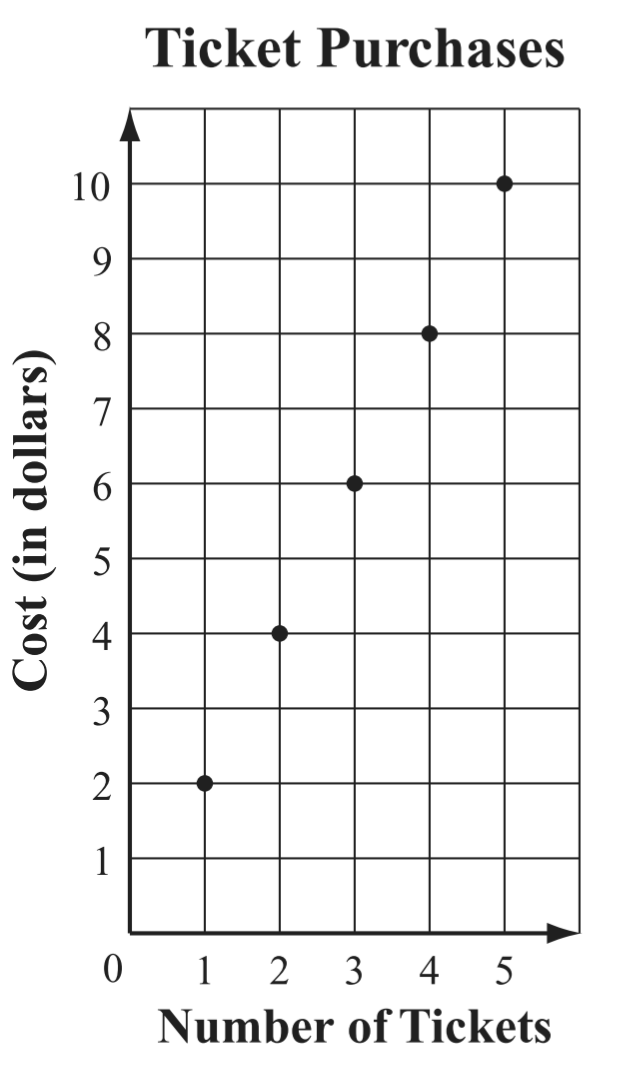
\includegraphics[width=0.8\linewidth]{ProportionalRelationships2}

\leavevmode\\\relax 
As the number of tickets purchased increases by 1,
how does the cost of the ticket purchase change?
\leavevmode\\\relax 
A. It increases by \$0.50.
\leavevmode\\\relax 
B. It increases by \$1.00.
\leavevmode\\\relax 
C. It increases by \$2.00.
\leavevmode\\\relax 
D. It increases by \$4.00.
\leavevmode\\\relax 



\smallskip
\goodbreak
\hrule
\nobreak

%%% BEGIN PROBLEM PREAMBLE
{\bf 24.} (1 point) \ifdim\lastskip=\pgmlMarker
  \let\pgmlPar=\relax
 \else
  \let\pgmlPar=\par
  \vadjust{\kern3pt}%
\fi

%%%%%%%%%%%%%%%%%%%%%%%%%%%%%%%%%%%%%%
%
%    definitions for PGML
%

\ifx\pgmlCount\undefined  % do not redefine if multiple files load PGML.pl
  \newcount\pgmlCount
  \newdimen\pgmlPercent
  \newdimen\pgmlPixels  \pgmlPixels=.5pt
\fi
\pgmlPercent=.01\hsize

\def\pgmlSetup{%
  \parskip=0pt \parindent=0pt
%  \ifdim\lastskip=\pgmlMarker\else\par\fi
  \pgmlPar
}%

\def\pgmlIndent{\par\advance\leftskip by 2em \advance\pgmlPercent by .02em \pgmlCount=0}%
\def\pgmlbulletItem{\par\indent\llap{$\bullet$ }\ignorespaces}%
\def\pgmlcircleItem{\par\indent\llap{$\circ$ }\ignorespaces}%
\def\pgmlsquareItem{\par\indent\llap{\vrule height 1ex width .75ex depth -.25ex\ }\ignorespaces}%
\def\pgmlnumericItem{\par\indent\advance\pgmlCount by 1 \llap{\the\pgmlCount. }\ignorespaces}%
\def\pgmlalphaItem{\par\indent{\advance\pgmlCount by `\a \llap{\char\pgmlCount. }}\advance\pgmlCount by 1\ignorespaces}%
\def\pgmlAlphaItem{\par\indent{\advance\pgmlCount by `\A \llap{\char\pgmlCount. }}\advance\pgmlCount by 1\ignorespaces}%
\def\pgmlromanItem{\par\indent\advance\pgmlCount by 1 \llap{\romannumeral\pgmlCount. }\ignorespaces}%
\def\pgmlRomanItem{\par\indent\advance\pgmlCount by 1 \llap{\uppercase\expandafter{\romannumeral\pgmlCount}. }\ignorespaces}%

\def\pgmlCenter{%
  \par \parfillskip=0pt
  \advance\leftskip by 0pt plus .5\hsize
  \advance\rightskip by 0pt plus .5\hsize
  \def\pgmlBreak{\break}%
}%
\def\pgmlRight{%
  \par \parfillskip=0pt
  \advance\leftskip by 0pt plus \hsize
  \def\pgmlBreak{\break}%
}%

\def\pgmlBreak{\\}%

\def\pgmlHeading#1{%
  \par\bfseries
  \ifcase#1 \or\huge \or\LARGE \or\large \or\normalsize \or\footnotesize \or\scriptsize \fi
}%

\def\pgmlRule#1#2{%
  \par\noindent
  \hbox{%
    \strut%
    \dimen1=\ht\strutbox%
    \advance\dimen1 by -#2%
    \divide\dimen1 by 2%
    \advance\dimen2 by -\dp\strutbox%
    \raise\dimen1\hbox{\vrule width #1 height #2 depth 0pt}%
  }%
  \par
}%

\def\pgmlIC#1{\futurelet\pgmlNext\pgmlCheckIC}%
\def\pgmlCheckIC{\ifx\pgmlNext\pgmlSpace \/\fi}%
{\def\getSpace#1{\global\let\pgmlSpace= }\getSpace{} }%

{\catcode`\ =12\global\let\pgmlSpaceChar= }%
{\obeylines\gdef\pgmlPreformatted{\par\small\ttfamily\hsize=10\hsize\obeyspaces\obeylines\let^^M=\pgmlNL\pgmlNL}}%
\def\pgmlNL{\par\bgroup\catcode`\ =12\pgmlTestSpace}%
\def\pgmlTestSpace{\futurelet\next\pgmlTestChar}%
\def\pgmlTestChar{\ifx\next\pgmlSpaceChar\ \pgmlTestNext\fi\egroup}%
\def\pgmlTestNext\fi\egroup#1{\fi\pgmlTestSpace}%

\def^^M{\ifmmode\else\space\fi\ignorespaces}%
%%%%%%%%%%%%%%%%%%%%%%%%%%%%%%%%%%%%%%

%%% END PROBLEM PREAMBLE
What expression is the result when \(2a - 5\)
subtracted from \(3a + 3\) ? Put your answer in simplest (standard) form.

\smallskip
\par 
  \mbox{\parbox[t]{25ex}{\hrulefill}}


\ifdefined\nocolumns\else \end{multicols}\fi


\noindent {\tiny Generated by \copyright WeBWorK, http://webwork.maa.org, Mathematical Association of America}

 \ifdefined\nocolumns\else \begin{multicols}{2}
\columnwidth=\linewidth \fi



\end{multicols}
\vfill
\end{document}
